\chapter{Trace Encoder Output Packets} \label{packets}

The bulk of this section describes the payload of packets output from the Trace Encoder.  
The infrastructure used to transport these packets is outside the scope of this document, and
as such the manner in which packets are encapsulated for transport is not specified.
However, the following information must be provided to the encapsulator:

\begin{itemize}
  \item The packet type;
  \item The packet length, in bytes;
  \item The packet payload.
\end{itemize}

Two example transport schemes are the UltraSoC Messaging Infrastructure, and the Arm Trace Bus.
Figure~\ref{fig:packet-format} shows the encapsulation used for the UltraSoC infrastructure:
\begin{itemize}
  \item The header byte contains a 5-bit field specifying the payload length in bytes, a 2-bit
    field indicating the "flow" (destination routing indicator), and a bit to indicate whether
    an optional 16-bit timestamp is present;
  \item The index field indicates the source of the packet.  The number of bits is system dependent,
    And the initial value emitted by the trace encoder is zero (it gets adjusted as it propagates 
    through the infrastructure);
  \item An optional 2-byte timestamp;
  \item The packet payload.
\end{itemize}

\begin{figure}[h]
  \begin{center}
    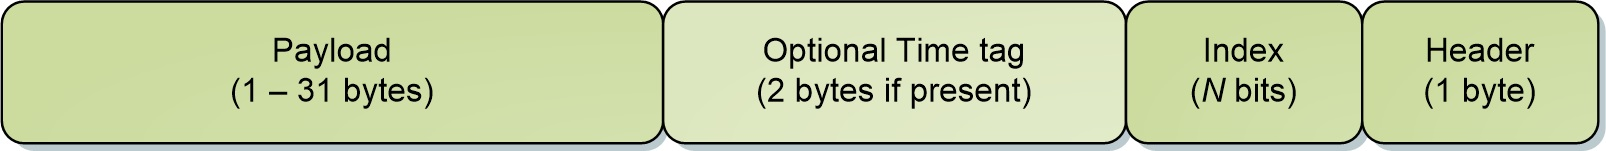
\includegraphics[height=1cm, width=9cm]{newPacket.jpg}
    \caption{Example Encapsulated Packet Format}
    \label{fig:packet-format}
  \end{center}
\end{figure}


Alternatively, for ATB, the source of the packet is indicated by the \textbf{ATID} bus field, and there is
no equivalent of "flow", so an example encapsulation might be:
\begin{itemize}
  \item A 5-bit field specifying the payload length in bytes
  \item A bit to indicate whether an optional 16-bit timestamp is present;
  \item An optional 2-byte timestamp;
  \item The packet payload.
\end{itemize}
It may be desirable for packets to start aligned to an ATB word, in which the \textbf{ATBYTES} bus field
in the last beat of a packet can be used to indicate the number of valid bytes.

The remainder of this section describes the contents of the payload
portion which should be independent of the infrastructure.  In each table, the fields are listed in
transmission order: first field in the table is transmitted first, and multi-bit fields are 
transmitted LSB first.

This packet payload format is used to output encoded instruction
trace.  Three different formats are used according to the needs of the
encoding algorithm. The following tables show the format of the
payload - i.e. excluding any encapsulation.

In order to achieve best performance, actual packet lengths may be adjusted using 'sign based compression'.
At the very minimum this should be applied to the address field of format 1 and 2 packets, but ideally will 
be applied to the whole packet, regardless of format.  This technique eliminates identical bits from the most 
significant end of the packet, and adjusts the length of the packet accordingly.  A decoder receiving this 
shortened packet can reconstruct the original full-length packet by sign-extending from the most significant
received bit.  An example of how this technique is used to choose between address formats is given in 
Section~\ref{addresses}.  The same principle can be applied to the entire packet, and the length (typically 
given in bytes) adjusted accordingly.

Where the payload length given in the following tables, or after applying sign-based compression, is not a 
multiple of whole bytes in length, the payload must be sign-extended to the nearest byte boundary.

Whilst offering maximum encoding efficiency, variable length packets can present some challenges,
specifically in terms of identifying where the boundaries between packets occur either when packed
packets are written to memory, or when packets are streamed offchip via a communications channel.  Two 
potential solutions to this are as follows:

\begin{itemize}
  \item If the maximum packet payload length is 2\textsuperscript{N}-1 (for example, if N is 5, then the maximum length is
    31 bytes), and the minimum packet payload length is 1, then a sequence of at least 2\textsuperscript{N} zero 
    bytes cannot occur within a packet payload, and therefore the first non-zero byte seen after a sequence of 
    at least 2\textsuperscript{N} zero bytes must be the first byte of a packet.  This approach can be used for
    alignment in either memory or a data stream;
  \item An alternative approach suitable for packets written to memory is to divide memory into blocks of M bytes
    (e.g. 1kbyte blocks), and write packets to memory such that the first byte in every block is always the first
    byte of a packet.  This means packets cannot span block boundaries, and so zero bytes must be used to pad between 
    the end of the last message in a block and the block boundary.
\end{itemize}

\begin{table}[htp]
  \centering
  \caption{Packet Payload Format 1 - with address}
  \label{tab:te_inst0-1-addr}
  \begin{tabulary}{\textwidth}{|l|p{35mm}|p{80mm}|}
    \hline
    {\bf Field name} & {\bf Bits} & {\bf Description} \\
    \hline
    \textbf{format}	& 2	& 01 (diff-delta): includes branch map and may include differential address\\
    \hline
    \textbf{branches} & 5 & Number of valid bits in branch-map. The length of branch-map is determined as follows: \newline
    0:      (cannot occur for this format) \newline
    1: 	1 bit \newline
    2-9: 	9 bits \newline
    10-17: 	17 bits \newline
    18-25: 	25 bits \newline
    26-31: 	31 bits \newline
    For example if branches = 12, the branch-map is 17 bits long, and the 12 LSBs are valid. \newline
    In most cases when the branch map is full there is no need to report an address,
    and this is indicated by setting branches to 0.  The exception to this is when 
    the instruction immediately prior to the final branch causes an uninferable discontinuity.\\
    \hline
    \textbf{branch\_map} & Determined by \newline 
                 \textbf{branches} field. & 
                 An array of bits indicating whether branches are taken or not.\newline
    Bit 0 represents the oldest branch instruction executed.   For each bit: \newline
    0: branch taken \newline
    1: branch not taken \\
    \hline
    \textbf{address}	& \textit {iaddress\_width\_p - iaddress\_lsb\_p} & 
                Differential instruction address.\\
    \hline
    \textbf{updiscon}	& 1 & 
                If the value of this bit is different from the MSB of \textbf{address}, it indicates that this 
                packet is reporting the instruction following an uninferable discontinuity and is also the 
                instruction before an exception, privilege change or resync 
                (i.e. it will be followed immediately by a format 3 \textit{te\_inst}).\\
    \hline
    \textbf{irfail}	& 1 & 
                If the value of this bit is different from \textbf{updiscon}, it indicates that this
                packet is reporting the instruction following a return because its address differs from 
                the predicted return address at the top of the implicit\_return return address stack.\\
    \hline
    \textbf{irdepth}	& \textit {call\_counter\_size\_p} & 
                If the value of \textbf{irfail} is different from \textbf{updiscon}, this field indicates 
                the number of entries on the return address stack (i.e. the entry number of the return that
                failed).  If \textbf{irfail} is the same value as \textbf{updiscon}, all bits in this field 
                will also be the same value as \textbf{updiscon}. \\
    \hline
  \end{tabulary}
\end{table}

\begin{table}[htp]
  \centering
  \caption{Packet Payload Format 1  - no address, branch map}
  \label{tab:te_inst0-1-noaddr-map}
  \begin{tabulary}{\textwidth}{|l|p{35mm}|p{80mm}|}
    \hline
    {\bf Field name} & {\bf Bits} & {\bf Description} \\
    \hline
    \textbf{format}	& 2	& 01 (diff-delta): includes branch map and may include differential address\\
    \hline
    \textbf{branches} & 5 & Number of valid bits in branch-map. The length of branch-map is determined as follows: \newline
    0:      31 bits, no \textbf{address} in packet \newline
    1-31: 	(cannot occur for this format) \\
    \hline
    \textbf{branch\_map} & 31 & 
                 An array of bits indicating whether branches are taken or not.\newline
    Bit 0 represents the oldest branch instruction executed.   For each bit: \newline
    0: branch taken \newline
    1: branch not taken \\
    \hline
    \textbf{branch\_fmt} & 2  & Both bits set to the same value as \textbf{branch\_map[MSB]} indicates that the
    preceding field is \textbf{branch\_map}. \\
    \hline
  \end{tabulary}
\end{table}

\begin{table}[htp]
  \centering
  \caption{Packet Payload Format 1 - no address, branch count}
  \label{tab:te_inst0-1-noaddr-count}
  \begin{tabulary}{\textwidth}{|l|p{35mm}|p{80mm}|}
    \hline
    {\bf Field name} & {\bf Bits} & {\bf Description} \\
    \hline
    \textbf{format}	& 2	& 01 (diff-delta): includes branch map and may include differential address\\
    \hline
    \textbf{branches} & 5 & Number of valid bits in branch-map. The length of branch-map is determined as follows: \newline
    0:      31 bits, no \textbf{address} in packet \newline
    31-1: 	(cannot occur for this format) \\
    \hline
    \textbf{branch\_count} & 16 & Count of the number of correctly predicted branches, minus 31. \\
    \hline
    reserved & 15 & zero\\
    \hline
    \textbf{branch\_fmt} & 2 & Set to 01, indicates that the packet contains a \textbf{branch\_count} field, no
    \textbf{address} field, and that the next branch failed prediction. \\
    \hline
  \end{tabulary}
\end{table}

\begin{table}[htp]
  \centering
  \caption{Packet Payload Format 1 - differential address, branch count}
  \label{tab:te_inst0-1-addr-count}
  \begin{tabulary}{\textwidth}{|l|p{35mm}|p{80mm}|}
    \hline
    {\bf Field name} & {\bf Bits} & {\bf Description} \\
    \hline
    \textbf{format}	& 2	& 01 (diff-delta): includes branch map and may include differential address\\
    \hline
    \textbf{branches} & 5 & Number of valid bits in branch-map. The length of branch-map is determined as follows: \newline
    0:      31 bits, no \textbf{address} in packet \newline
    31-1: 	(cannot occur for this format) \\
    \hline
    \textbf{branch\_count} & 16 & Count of the number of correctly predicted branches, minus 31. \\
    \hline
    \textbf{address (LSBs)}	& 15 & 
                15 LSBs of differential instruction address.\\
    \textbf{branch\_fmt} & 2 & Set to 10, indicates that the packet contains a \textbf{branch\_count} field and
     an \textbf{address} field. This will be the case if the packet is output because it is necessary to report an
     address (e.g. following an updiscon, or if the next instruction is an exception), or because \textbf{branch\_count} 
     has reached 0xffff).\\
    \hline
    \textbf{bpsuccess} & 1 & This bit will be 1 if the most recent branch was predicted correctly. \\
    \hline
    \textbf{updiscon}	& 1 & 
                If the value of this bit is different from \textbf{bpfail}, it indicates that this 
                packet is reporting the instruction following an uninferable discontinuity and is also the 
                instruction before an exception, privilege change or resync 
                (i.e. it will be followed immediately by a format 3 \textit{te\_inst}).\\
    \hline
    \textbf{irfail}	& 1 & 
                If the value of this bit is different from \textbf{updiscon}, it indicates that this
                packet is reporting the instruction following a return because its address differs from 
                the predicted return address at the top of the implicit\_return return address stack.\\
    \hline
    \textbf{irdepth}	& \textit {call\_counter\_size\_p} & 
                If the value of \textbf{irfail} is different from \textbf{updiscon}, this field indicates 
                the number of entries on the return address stack (i.e. the entry number of the return that
                failed).  If \textbf{irfail} is the same value as \textbf{updiscon}, all bits in this field 
                will also be the same value as \textbf{updiscon}. \\
    \hline
    \textbf{address (MSBs)}	& \textit {iaddress\_width\_p - iaddress\_lsb\_p - 15} & 
                MSBs of the differential instruction address.\\
    \hline
  \end{tabulary}
\end{table}


\begin{table}[!h]
  \centering
  \caption{Packet Payload Format 2}
  \label{tab:te_inst2}
  \begin{tabulary}{\textwidth}{|l|p{35mm}|p{80mm}|}
    \hline
    {\bf Field name} & {\bf Bits} & {\bf Description} \\
    \hline
    \textbf{format}	& 2	& 10 (addr-only): differential address and no branch map\\
    \hline
    \textbf{address} & \textit {iaddress\_width\_p - iaddress\_lsb\_p} & 
              Differential instruction address.\\ 
    \hline
    \textbf{updiscon}	& 1 & 
                If the value of this bit is different from the MSB of \textbf{address}, it indicates that this 
                packet is reporting the instruction following an uninferable discontinuity and is also the 
                instruction before an exception, privilege change or resync 
                (i.e. it will be followed immediately by a format 3 \textit{te\_inst}).\\
    \hline
    \textbf{irfail}	& 1 & 
                If the value of this bit is different from \textbf{updiscon}, it indicates that this
                packet is reporting the instruction following a return because its address differs from 
                the predicted return address at the top of the implicit\_return return address stack.\\
    \hline
    \textbf{irdepth}	& \textit {call\_counter\_size\_p} & 
                If the value of \textbf{irfail} is different from \textbf{updiscon}, this field indicates 
                the number of entries on the return address stack (i.e. the entry number of the return that
                failed).  If \textbf{irfail} is the same value as \textbf{updiscon}, all bits in this field 
                will also be the same value as \textbf{updiscon}. \\
    \hline
  \end{tabulary}
\end{table}

\begin{table}[htp]
  \centering
  \caption{Packet Payload Format 3, subformat 0}
  \label{tab:te_inst3}
  \begin{tabulary}{\textwidth}{|l|p{35mm}|p{80mm}|}
    \hline
    {\bf Field name} & {\bf Bits} & {\bf Description} \\
    \hline
    \textbf{format} & 2 & 11 (sync): synchronisation\\
    \hline
    \textbf{subformat} & 2 & 00 (start): Start of tracing, or resync \\
    \hline
    \textbf{context} &  \textit {context\_width\_p}, 
               or 0 if \textit {nocontext\_p} is 1 & 
               The instruction context \\
    \hline
    \textbf{privilege} & \textit {privilege\_width\_p} & 
                The current privilege level \\
    \hline
    \textbf{address} & \textit {iaddress\_width\_p - iaddress\_lsb\_p} & 
              Full instruction address.  Address alignment is determined by \textit {iaddress\_lsb\_p} Address must be left shifted in order to recreate original byte address \\
    \hline
    \textbf{branch} & 1 & If the address points to a branch instruction, the branch is not taken if the value of this bit is different from the MSB of \textbf{address}. 
    Set to the same value as the MSB of \textbf{address} if the branch is taken or the instruction is not a branch. \\
    \hline
  \end{tabulary}
\end{table}

\begin{table}[htp]
  \centering
  \caption{Packet Payload Format 3, subformat 1}
  \label{tab:te_inst3}
  \begin{tabulary}{\textwidth}{|l|p{35mm}|p{80mm}|}
    \hline
    {\bf Field name} & {\bf Bits} & {\bf Description} \\
    \hline
    \textbf{format} & 2 & 11 (sync): synchronisation\\
    \hline
    \textbf{subformat} & 2 & 01 (exception): Exception cause and trap handler address\\
    \hline
    \textbf{context} &  \textit {context\_width\_p}, 
               or 0 if \textit {nocontext\_p} is 1 & 
               The instruction context \\
    \hline
    \textbf{privilege} & \textit {privilege\_width\_p} & 
                The current privilege level \\
    \hline
    \textbf{address} & \textit {iaddress\_width\_p - iaddress\_lsb\_p} & 
              Full instruction address.  Address alignment is determined by \textit {iaddress\_lsb\_p} Address must be left shifted in order to recreate original byte address \\
    \hline
    \textbf{ecause} & \textit {ecause\_width\_p} & 
             Exception cause \\
    \hline
    \textbf{interrupt} & 1 & 
                Interrupt \\
    \hline
    \textbf{tval} & \textit {iaddress\_width\_p}, 
           or 0 if \textit {notval\_p} is 1 & 
           Trap value \\
    \hline
    \textbf{branch} & 1 & If the address points to a branch instruction, the branch is not taken if the value of this bit is different from the MSB of \textbf{tval}. 
    Set to the same value as the MSB of \textbf{tval} if the branch is taken or the instruction is not a branch. \\
    \hline
  \end{tabulary}
\end{table}

\begin{table}[htp]
  \centering
  \caption{Packet Payload Format 3, subformat 2}
  \label{tab:te_inst3}
  \begin{tabulary}{\textwidth}{|l|p{35mm}|p{80mm}|}
    \hline
    {\bf Field name} & {\bf Bits} & {\bf Description} \\
    \hline
    \textbf{format} & 2 & 11 (sync): synchronisation\\
    \hline
    \textbf{subformat}  & 2 & 10 (context): Context change \\
    \hline
    \textbf{context} &  \textit {context\_width\_p} & The instruction context \\
      \hline
  \end{tabulary}
\end{table}

\begin{table}[htp]
  \centering
  \caption{Packet Payload Format 3, subformat 3}
  \label{tab:te_inst3}
  \begin{tabulary}{\textwidth}{|l|p{35mm}|p{80mm}|}
    \hline
     {\bf Field name} & {\bf Bits} & {\bf Description} \\
     \hline
     \textbf{format} & 2 & 11 (sync): synchronisation\\
     \hline
     \textbf{subformat}  & 2 & 11 (support): Supporting information for the decoder \\
     \hline
     \textbf{enable} & 1 & Indicates if encoder is enabled\\
     \hline
     \textbf{encoder\_mode} & N & Identifies trace algorithm\newline
       Details implementation dependent.  Currently Branch trace is the only mode defined.\\
     \hline
     \textbf{qual\_status} & 2 & Indicates qualification status\newline
       00 (no\_change): No change to filter qualification \newline
       01 (ended\_rep): Qualification ended, preceding \textbf{te\_inst} sent explicitly to indicate last qualification instruction\newline
       10: (packet\_lost): One or more packets lost.\newline
       11 : (ended\_ntr): Qualification ended, no unreported instructions (so preceeding \textbf{te\_inst} would have been sent anyway, even if it wasn't the last qualified instruction)\\
     \hline
     \textbf{options} & N & Values of all run-time configuration bits\newline
       Number of bits and definitions implementation dependent.  Examples might be\newline
       - 'implicit return' Don't report function return addresses \newline
       - 'implicit exception' Exclude address from format 3, sub-format 1 \textit{te\_inst} packets if trap vector can be determined from \textit{ecause field}\newline
       - 'branch prediction' Branch predictor enabled\newline
       - 'full address' Always output full addresses (SW debug option)\\
       \hline
  \end{tabulary}
\end{table}

\section {Further notes on packet format details}

Some of the packet fields warrant further explanation.

\subsection{Format 3 \textbf{branch} field}

This bit indicates the taken/not taken status in the case where the reported address points to a branch instruction.
Overall efficiency would be slightly improved if this bit was removed, and the branch status was instead 
"carried over" and reported in the next \textit{te\_inst} packet.  This was considered, but there are several
pathological cases where this approach fails.  Consider for example the situation where the first instruction
that matches the filtering criteria is a branch, and this is then followed immediately by an exception.  This
results in format 3 packets being generated on two consecutive cycles.  The second packet does not contain a branch
map, so there is no way to report the branch status of the 1st branch, apart from by inserting a format 1 packet in 
between.  There are two issues with this:

\begin{itemize}
  \item It would require the generation of 2 packets on the same cycle, which adds significant additional complexity
    to the encoder;
  \item It would complicate the algorithm shown in~\ref{fig:algo}. 
\end{itemize}

This bit is encoded so that most of the time it will take the same value as the MSB of the preceding field, and will
therefore compress away, in order to minimize the efficiency impact.  Branches are unlikely to be reported using a
format 3 packet apart from if the 1st traced instruction is a branch, or if the instruction reported when the 
resync timer expires is a branch.

\subsection{Format 1/2 \textbf{updiscon} field}

This bit is encoded so that most of the time it will take the same value as the MSB of the \textbf{address} field,
and will therefore compress away, having no impact on the encoding efficiency.  It is required in order to cover a
pathological case where otherwise the decoding software would not be able to reconstruct the program execution
unambiguously.  Consider the following code fragment:

looplabel~~-~4: \textbf{\textit{opcode A}} \newline
looplabel~~~~~: \textbf{\textit{opcode B}} \newline
looplabel~+~4: \textbf{\textit{opcode C}} \newline
~~: \newline
looplabel~+~N: \textbf{\textit{JALR}} \# Jump to looplabel\newline

This is a loop with an indirect jump back to the next iteration.  This is an uninferable discontinuity, and will be
reported via a format 1 or 2 packet.  Note however that the initial entry into the loop is fall-through from the
instruction at looplabel - 4, and will not be reported explicitly.  This means that when reconstructing the execution 
path of the program, the looplabel address is encountered twice.  On first glance, it appears that the decoder can determine
when it reaches the loop label for the 1st time that this is not the end of execution, because the preceding
instruction was not one that can cause an uninferable discontinuity.  It can therefore continue reconstructing the 
execution path until it reaches the \textbf{\textit{JALR}}, from where it can deduce that \textbf{\textit{opcode B}} at
looplabel is the final retired instruction.  However, there are circumstances where this approach 
does not work.  For example, consider the case where there is an exception at looplabel + 4.  In this case, the decoder
cannot tell whether this occurred during the 1st or 2nd loop iterations, without additional information from the 
encoder.  This is the purpose of the \textbf{updiscon} field.  In more detail:

There are three scenarios to consider:

\begin{enumerate}
  \item Code executes through to the end of the 1st loop iteration, and the encoder reports looplabel using format 1/2 following 
    the \textbf{\textit{JALR}}, then carries on executing the 2nd pass of the loop.  In this case \textbf{updiscon} == \textbf{address[MSB]}.  
    The next packet will be a format 1/2;
  \item Code executes through to the end of the 1st loop iteration, but there is an exception, privilege change or resync at
    the instruction following the \textbf{\textit{JALR}} (i.e. at looplabel + 4).  In this case, the encoder reports looplabel using 
    format 1/2 following the \textbf{\textit{JALR}}, with \textbf{updiscon} == !\textbf{address[MSB]}, and the next packet is a 
    format 3;
  \item An exception occurs after the 1st execution of looplabel.  In this case, the encoder reports looplabel using format 0/1/2 and again,
    \textbf{updiscon} == \textbf{address[MSB]}, and the next packet is a format 3.
\end{enumerate}

Looking at this from the perspective of the decoder, the decoder receives a format 1/2 reporting the address of the 1st instruction in the 
loop (looplabel).  It follows the execution path from the last reported address, until it reaches looplabel.  Because looplabel is not 
preceded by an uninferable discontinuity, it must take the value of \textbf{updiscon} into consideration, and may need to wait for the 
next packet in order to determine whether it has reached the final retired instruction:
\begin{itemize}  
  \item If \textbf{updiscon} == !\textbf{address[MSB]}, this indicates case 2.  The decoder must continue until it encounters 
    looplabel a 2nd time;
  \item If \textbf{updiscon} == \textbf{address[MSB]}, the decoder cannot yet distinguish cases 1 and 3, and must wait for the 
    next packet.
    \begin{itemize}
      \item If the next packet is a format 3, this is case 3.  The decoder has already reached the correct instruction;
      \item If the next packet is a format 1/2, this is case 1.  The decoder must continue until it encounters 
        looplabel a 2nd time.
    \end{itemize}
\end{itemize}

This example uses an exception at looplabel + 4, but anything that could cause a format 3 for looplabel + 4 would result in 
the same behavior: a privilege change, or the expiry of the resync timer.  It could also occur if looplabel was the last
traced instruction (because tracing was disabled for some reason).  See next section for further discussion of this point.

\subsection{Format 1 \textbf{branch\_fmt} field}

This is encoded so that it will take the same value as the MSB of the \textbf{branch\_map} field, so that extra bits are
only required when reporting predicted branch counts, and reporting a branch map is unaffected.  Although there are 15
unused bits when reporting a branch count without address, branch counts will by their nature be reported much less 
frequently, so this is not a significant cost.  Furthermore, even for the most pathological case (32 correctly predicted 
branches followed by a misprediction), the total number of bits used is still fewer than if using just the branch map
format.

\subsection{Format 1 \textbf{bpsuccess} field}
This bit is encoded so that most of the time it will take the same value as the MSB of the \textbf{branch\_fmt} field,
and will therefore compress away, having no impact on the encoding efficiency.  When a branch count is reported without 
an address it is because a branch has failed the prediction.  However, when an address is reported along with
a branch count, it will be because the packet was initiated by an uninferable discontinuity, an exception, or because a
branch has been encountered when the number of correctly predicted branches is 0xffff.  For the latter case, the 
reported address will always be for a branch, and in the former cases it may be.  If it is a branch, it is necessary to 
be explicit about whether or not the prediction was met or not.

\subsection{Format 1/2 \textbf{irfail} and \textbf{irdepth} fields}
These bit are encoded so that most of the time they will take the same value as the \textbf{updiscon} field,
and will therefore compress away, having no impact on the encoding efficiency.  If implicit\_return mode is enabled, and
the encoder maintains a stack of predicted return addresses that are compared with the actual return addresses, then
a \textit{te\_inst} packet will be generated if a misprediction occurs.  In order to correctly reconstruct the 
execution path of the program, the decoder will need to know which return it was that failed.  If a return is reported
because the return address stack is empty, these fields will take the same value as the \textbf{updiscon} field.

\subsection{Format 3 subformat 3 \textbf{qual\_status} field}

When tracing ends, the encoder reports the address of the last traced instruction, and follows this with a format 3, 
subformat 3 (supporting information) packet.  Two codes are provided for indicating that tracing has ended: 
\textbf{ended\_rep} and \textbf{ended\_ntr}.  This relates to exactly the same ambiguous case described in the previous
section, and in principle, the mechanism described in that section can be used to disambiguate when the last traced
instruction is at looplabel + 4.  However, that mechanism relies on knowing when creating the format 1/2 packet, that 
a format 3 packet will be generated from the next instruction.  This is possible because the encoding algorithm uses 
a 3-stage pipe with access to the previous, current and next instructions.  However, decoding that the next instruction
is a priviledge change or exception is straightforward, but determining whether the next instruction meets the filtering
criteria is much more involved, and this information won't typically be available, at least not without adding an
additional pipeline stage, which is expensive.  This means a different mechanism is required, and that is provided
by having two codes to indicate that tracing has ended:

\begin{itemize}
  \item \textbf{ended\_rep} indicates that the preceding packet would not have been issued if tracing hadn't ended, 
    which means that tracing stopped after executing looplabel in the 1st loop iteration;
  \item \textbf{ended\_ntr} indicates that the preceding packet would have been issued anyway, 
    which means that tracing stopped after executing looplabel in the 2nd loop iteration;
\end{itemize}

If the encoder implementation does have early access to the filtering results, and the designer chooses to use the
\textbf{updiscon} when thet last qualified instruction is also the instruction following an uninferable PC discontinuity,
loss of qualification shoujld always be indicated using \textbf{ended\_ntr}.
